% sips -s format png your_pdf_file.pdf --out your_png_file.png

\documentclass[tikz,border=0mm]{standalone}

\usepackage{amsmath}
\usepackage{graphicx}
\usepackage[T1]{fontenc}
\renewcommand\familydefault{\sfdefault} 

\usetikzlibrary{arrows,shapes,calc,math,decorations.fractals,patterns,backgrounds,decorations.markings,decorations.pathmorphing}

\tikzset{point/.style={fill,circle,inner sep=1.5pt}}
\tikzset{vector/.style={-triangle 45, line width=1pt}}
\tikzset{dblarrow/.style={latex'-latex'}}
\tikzset{partial ellipse/.style args={#1:#2:#3}{insert path={+ (#1:#3) arc (#1:#2:#3)}}}
\tikzset{xaxis/.style={-stealth',red,line width=1pt}}
\tikzset{yaxis/.style={-stealth',green!80!black,line width=1pt}}
\tikzset{zaxis/.style={-stealth',blue,line width=1pt}}
\renewcommand{\vec}{\mathbf}

% FLow chart nodes
\tikzstyle{startstop} = [rectangle, rounded corners, minimum width=3cm, minimum height=1cm,text centered, draw=black, fill=red!30]
\tikzstyle{io} = [trapezium, trapezium stretches=true,trapezium left angle=70, trapezium right angle=110, minimum width=1cm, minimum height=1cm, text centered, draw=black, fill=blue!30]
\tikzstyle{process} = [rectangle, minimum width=3cm, minimum height=1cm, text centered, draw=black, fill=orange!30]
\tikzstyle{decision} = [diamond, aspect=2, minimum width=3cm, minimum height=1cm, text centered, draw=black, fill=green!30]
\tikzstyle{arrow} = [thick,->,>=stealth]

\begin{document}

% Logo

\begin{tikzpicture}
    \draw [rounded corners=0.25cm,line width=4pt,fill=blue!15!white] (-1.5, -1) rectangle ++(3, 1.75);
    \draw [line width=4pt] (-1.5,-0.7) -- ++(3, 0);
    \draw [line width=4pt,line cap=round] (-0.5,-1) -- ++(0,-0.33) (0.5,-1) -- ++(0,-0.33) (-1,-1.33) -- ++(2,0);
    \node {\Huge \verb!</>!};
    \node at (0,-2) {\Large \bf Programming Skills};
\end{tikzpicture}

% Spyder window
% \begin{tikzpicture}
%     \node {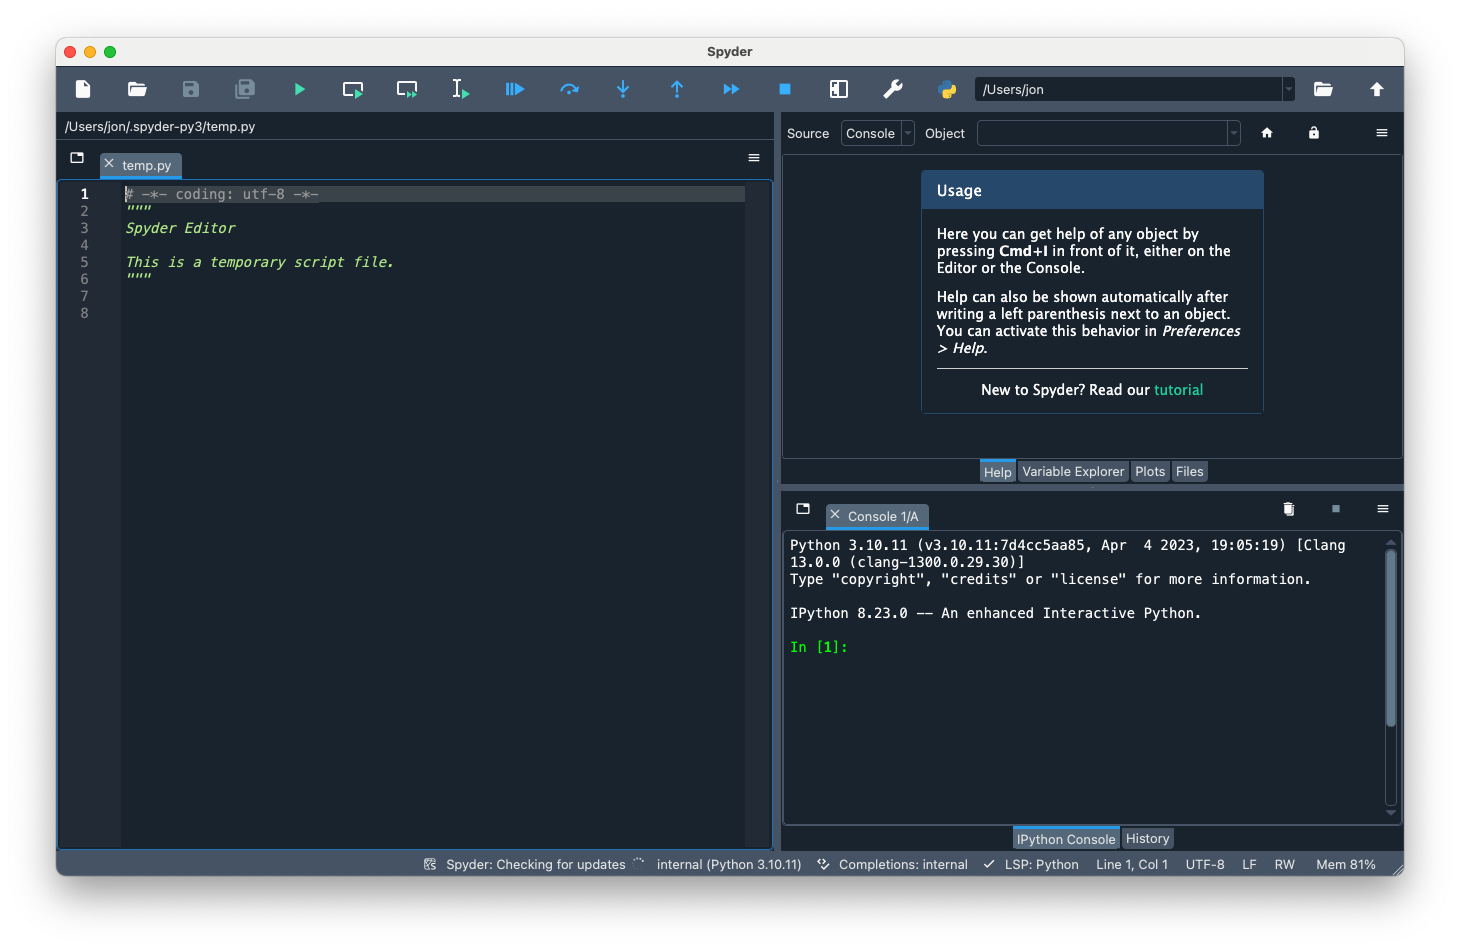
\includegraphics{../1_Spyder.png}};
%     \draw [red,line width=4pt] (2,-13.2) rectangle ++(21.7,12.5);
%     \node [red] at ($(2,-13.2)!0.5!(23.7,-1)$) {\Huge \bf Console pane};
%     \draw [green,line width=4pt] (-23.5, -13.2) rectangle ++(25,25);
%     \node [green] at ($(-23.5,-13.2)!0.5!(1.5,11.8)$) {\Huge \bf Editor pane};
% \end{tikzpicture}

% Function
% \begin{tikzpicture}[every node/.style={node distance=0.5cm}]
%     \node [draw,fill=blue!10,rectangle,rounded corners,text width=2cm,align=center,line width=1pt,minimum height=0.75cm] (function) {Function};
%     \node [left of=function,node distance=3cm] (input2) {input 2};
%     \node [above of=input2] (input1) {input 1};
%     \node [below of=input2] (input3) {input 3};
%     \node [right of=function,node distance=3cm,yshift=0.25cm] (output1) {output 1};
%     \node [right of=function,node distance=3cm,yshift=-0.25cm] (output2) {output 2};
%     \draw [->,shorten >= 2pt,line width=1pt] (input1.east) to (function);
%     \draw [->,shorten >= 2pt,line width=1pt] (input2) to (function);
%     \draw [->,shorten >= 2pt,line width=1pt] (input3.east) to (function);
%     \draw [->,shorten <= 2pt,line width=1pt] (function) to (output1.west);
%     \draw [->,shorten <= 2pt,line width=1pt] (function) to (output2.west);
% \end{tikzpicture}

\end{document}